% Auto-generated companion figure environment by academic-viz-stats
\begin{figure}[t]
\centering
\IfFileExists{figures/benchmark_statistical_evaluation.pdf}{
    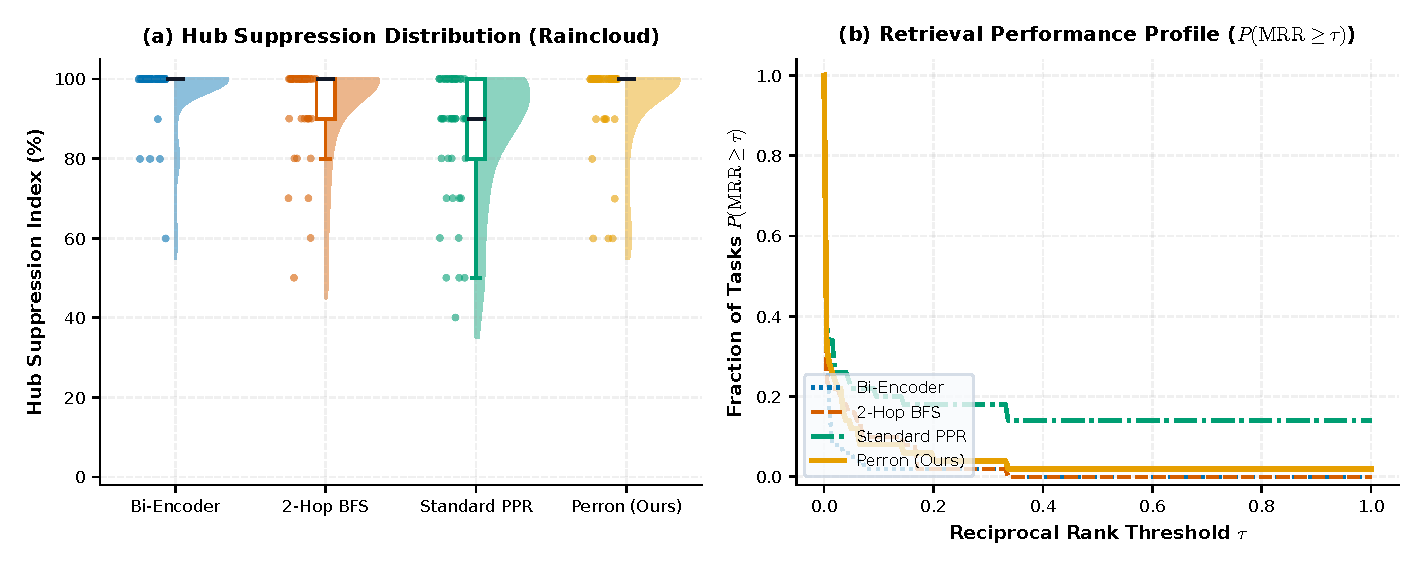
\includegraphics[width=\textwidth]{figures/benchmark_statistical_evaluation.pdf}
}{
    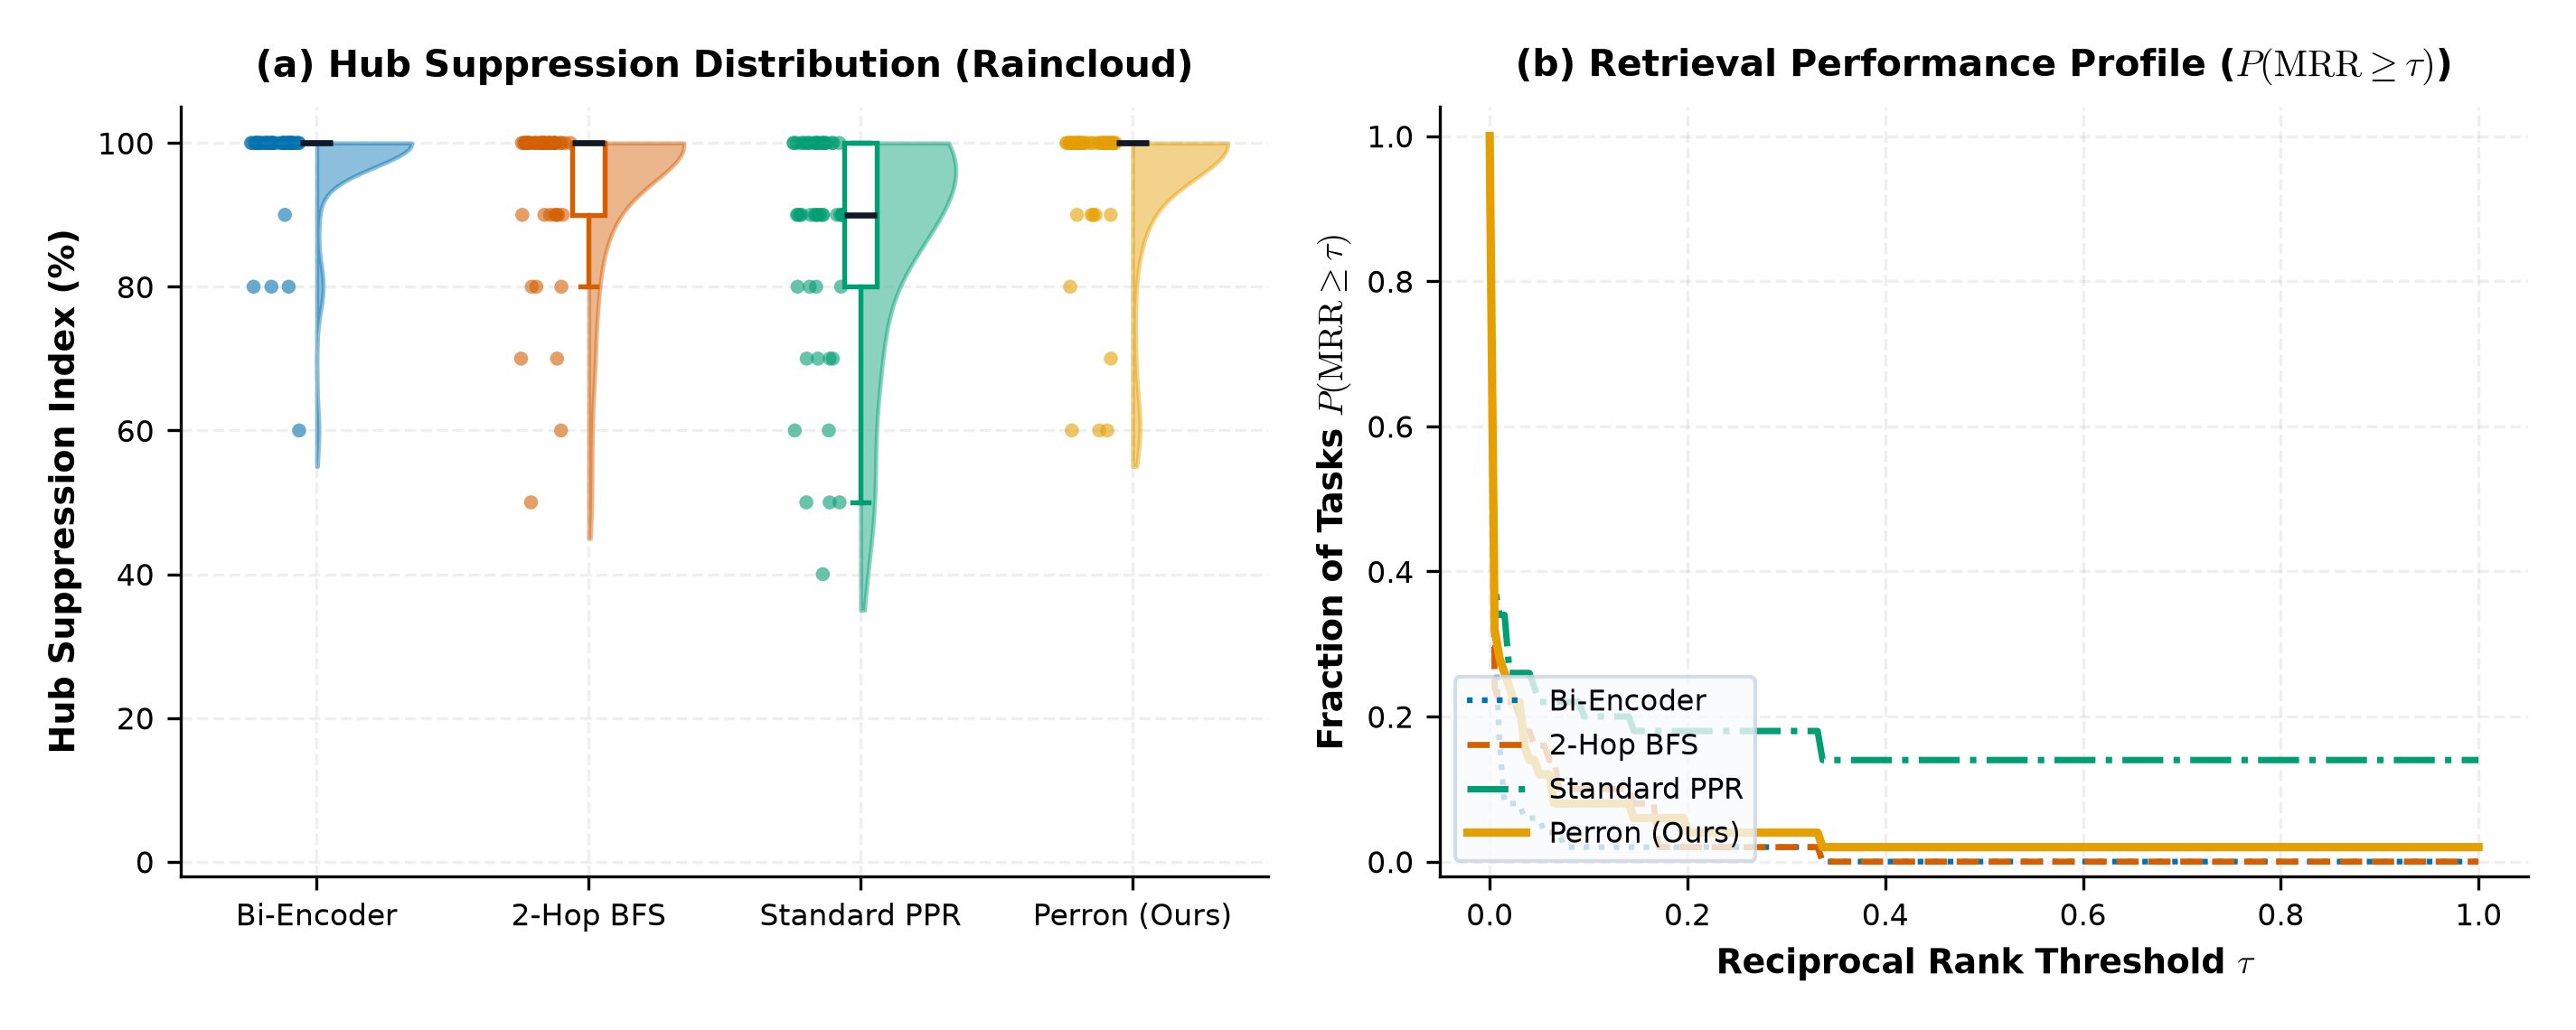
\includegraphics[width=\textwidth]{figures/benchmark_statistical_evaluation.png}
}
\caption{\textbf{Rigorous real repository retrieval and hub suppression benchmark evaluation.} (a) Raincloud plot showing the continuous distribution of the Hub Suppression Index (HSI) across 50 real SWE-bench Lite instances on scale-free Python repository dependency graphs (Requests and SymPy). Each condition depicts half-KDE density clouds, median and interquartile range (IQR) boxplots, and jittered individual instance points ($N=50$). Perron suppresses \PerronHSIMean\ of utility hubs, demonstrating a statistically significant improvement over Standard PPR (paired $t(\HSIDF) = \HSITValue$, $p \HSIPValue$, Cliff's $\delta = \HSICliffsDelta$). (b) Dolan--Mor\'e performance profile displaying the empirical cumulative distribution of Mean Reciprocal Rank ($P(\mathrm{MRR} \geq \tau)$) across thresholds $\tau \in [0, 1]$, illustrating the retrieval ranking distribution across thresholds.}
\label{fig:benchmark_statistical_evaluation}
\end{figure}
